% Section content template for individual Educative lessons
% This file contains the actual content for a specific section
% Generated from Educative API section content

% Section: Sequence Diagram for the Elevator System
% Section ID: 6423575504617472
% Section Slug: sequence-diagram-for-the-elevator-system
% Generated: 2025-12-11T14:08:37.335711

A sequence diagram is a great way to understand the interactions between different entities and objects in the system. There can be different sequence diagrams that we can create for our elevator system. In this lesson, we will create sequence diagrams for the following two interactions:

\begin{itemize}
\item
\protect\phantomsection\label{TUa_BJ0JS77gRm3LlZ4Zn}
\textbf{Elevator call:} The passenger calls the elevator.
\item
\protect\phantomsection\label{aJ9bHxUKwJgFdt0QrqVQX}
\textbf{Sequence challenge:} The passenger rides the elevator to a floor.
\end{itemize}

\subsection{Elevator call}\label{-xvkkT8V-VfJnKhLeJHMc}
\\
The sequence diagram for an elevator call should have the following actors and objects that will interact with each other:

\begin{itemize}
\item
\protect\phantomsection\label{KyrXYxhj7xn5QY7xpMpIz}
\textbf{Actor:}~\texttt{Passenger}
\item
\protect\phantomsection\label{Ccn6aN9FGMkBTfYPLKxLj}
\textbf{Objects:~}\texttt{HallButton},~\texttt{ElevatorSystem},~\texttt{Dispatcher},~\texttt{ElevatorCar}, and~\texttt{Door}
\end{itemize}
\\
Here are the steps in the elevator call interaction:

\begin{enumerate}
\item
\protect\phantomsection\label{-f92h4oN9c2NDXK9UnlZD}
The passenger presses the hall button to call the elevator.
\item
\protect\phantomsection\label{gv-p16zCO8N3uiYXjKBhl}
The hall button signals the elevator system to call an elevator car to the passenger's floor.
\item
\protect\phantomsection\label{RqQe4eCOdAFKSt5VhhUxs}
The elevator system checks for available cars (idle state) and ignores all cars in maintenance state.
\item
\protect\phantomsection\label{9FzpuJEldTidDM-a40-s_}
The elevator system informs the dispatcher to select the best car.
\item
\protect\phantomsection\label{2POINvqu6SH93msLk9KiQ}
The dispatcher returns the best car to the system.
\item
\protect\phantomsection\label{ns0K8r-BEia3cpfk1Gjf6}
The elevator system signals the elevator car to move to the passenger's floor.
\item
\protect\phantomsection\label{Z-r0WgTqGXKj_6zI5r9qO}
The elevator car signals the system when it arrives on the floor.
\item
\protect\phantomsection\label{tVKkKwvALF6M0VxCl9rNG}
The system signals the hall button that the elevator has arrived.
\item
\protect\phantomsection\label{Jx9X27S3hvrAkkFUDrwgS}
The hall button is unpressed.
\item
\protect\phantomsection\label{vBEieDHDYmke4U9vWkxwX}
The elevator system signals the doors to open.
\item
\protect\phantomsection\label{F5_bICd1HrMAhNfikxLjE}
The door opens for the passenger.
\end{enumerate}
\\
Based on the order above, the sequence diagram for an elevator call in the elevator system is given below.

\begin{figure}[htbp]
 \centering
 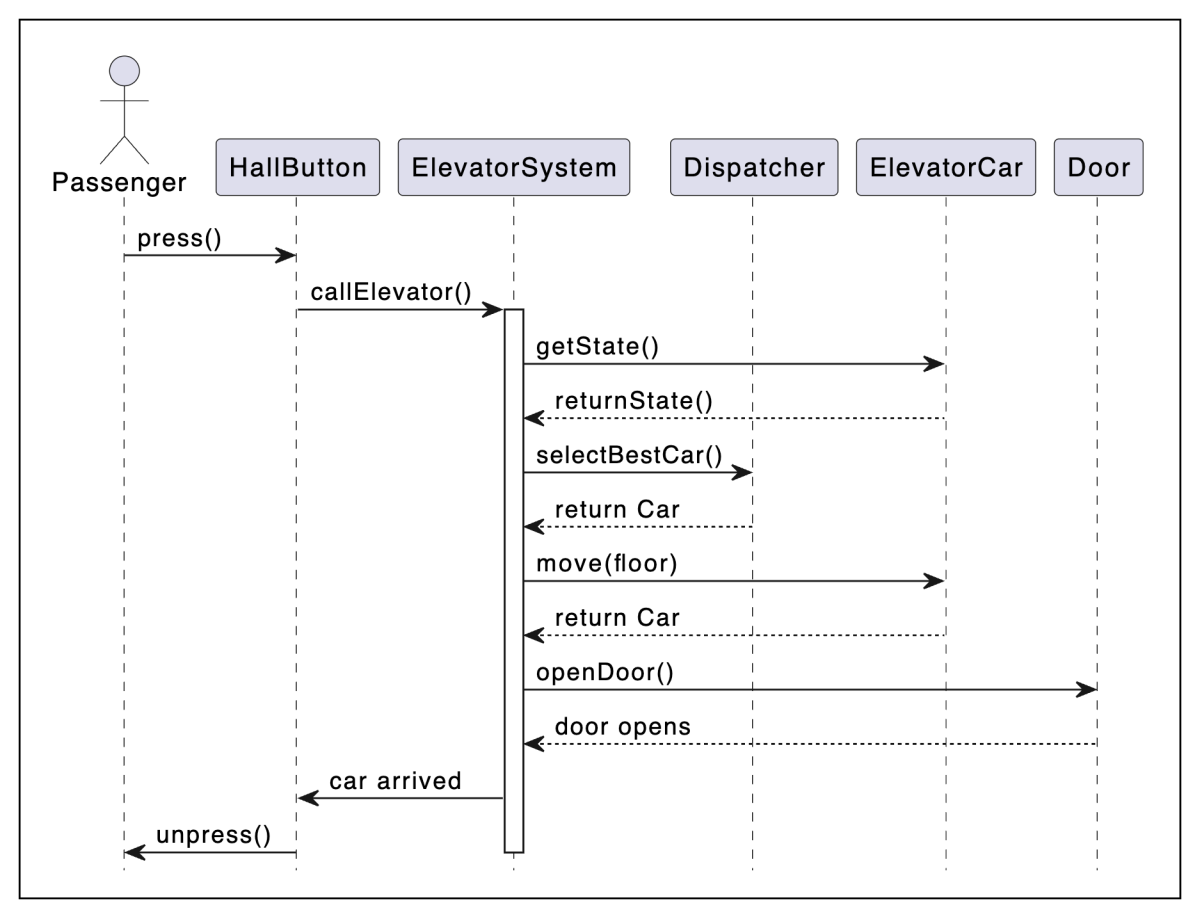
\includegraphics[width=0.5\textwidth]{Images/chapter_8/section_6423575504617472/6072783971680256.png}
 \caption{The sequence diagram for an elevator call}
\end{figure}

\subsection{Sequence challenge: Elevator ride}\label{Sequence-challenge-Elevator-ride}
\\
You will complete a sequence diagram for an elevator ride from one floor to another, assuming elevator cars are in the idle state. A skeleton of the sequence diagram for an elevator ride is given below:

\begin{figure}[htbp]
 \centering
 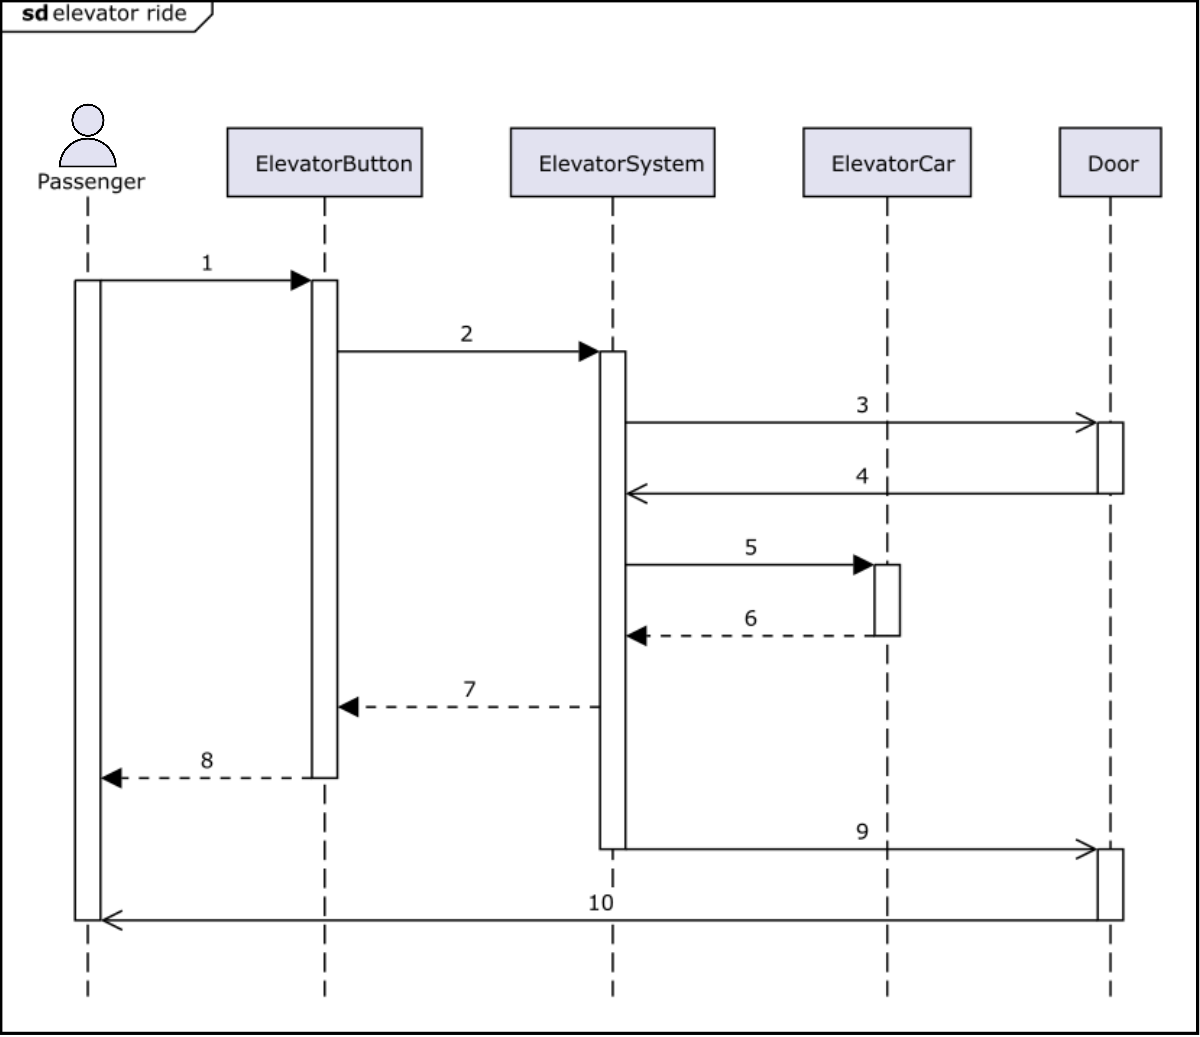
\includegraphics[width=0.5\textwidth]{Images/chapter_8/section_6423575504617472/6664402719473664.png}
 \caption{The sequence diagram for an elevator ride}
\end{figure}

Notice that the arrows in the diagram above are numbered from 1 to 9. The boxes below are the messages between the actor(s) and object(s). Can you rearrange the messages below in the correct order so that they appear in the skeleton of the sequence diagram above?
\begin{quote}
\textbf{Note:} If you're stuck, click the ``Show Solution'' button.
\end{quote}

Alternatively, you can also click the ``Show complete diagram'' button below to see the complete sequence diagram for the elevator ride interaction.

Next, let's look at the elevator system activity diagrams to understand the system's control flow.

% End of section content